\documentclass[12pt, notitlepage, final]{article} 

\newcommand{\name}{Vince Coghlan}

%\usepackage[dvips]{graphics,color}
\usepackage{amsfonts}
\usepackage{amssymb}
\usepackage{amsmath}
\usepackage{latexsym}
\usepackage{enumerate}
\usepackage{amsthm}
\usepackage{nccmath}
\usepackage{setspace}
\usepackage[pdftex]{graphicx}
\usepackage{epstopdf}
\usepackage[siunitx]{circuitikz}
\usepackage{tikz}
\usepackage{float}
\usepackage{cancel} 
\usepackage{setspace}
\usepackage{overpic}
\usepackage{mathtools}
\usepackage{listings}
\usepackage{color}
\usepackage{qtree}
%\usepackage{gensymb}

\usetikzlibrary{calc}
\usetikzlibrary{matrix}
\usetikzlibrary{positioning}

\numberwithin{equation}{section}
\DeclareRobustCommand{\beginProtected}[1]{\begin{#1}}
\DeclareRobustCommand{\endProtected}[1]{\end{#1}}
\newcommand{\dbr}[1]{d_{\mbox{#1BR}}}
\newtheorem{lemma}{Lemma}
\newtheorem*{corollary}{Corollary}
\newtheorem{theorem}{Theorem}
\newtheorem{proposition}{Proposition}
\theoremstyle{definition}
\newtheorem{define}{Definition}
\newcommand{\column}[2]{
\left( \begin{array}{ccc}
#1 \\
#2
\end{array} \right)}

\newdimen\digitwidth
\settowidth\digitwidth{0}
\def~{\hspace{\digitwidth}}

\setlength{\parskip}{1pc}
\setlength{\parindent}{0pt}
\setlength{\topmargin}{-3pc}
\setlength{\textheight}{9.0in}
\setlength{\oddsidemargin}{0pc}
\setlength{\evensidemargin}{0pc}
\setlength{\textwidth}{6.5in}
\newcommand{\answer}[1]{\newpage\noindent\framebox{\vbox{{\bf ECEN 5018 Spring 2014} 
\hfill {\bf \name} \vspace{-1cm}
\begin{center}{Homework \#7}\end{center} } }\bigskip }

\DeclareMathOperator*{\argmin}{arg\,min}

%absolute value code
\DeclarePairedDelimiter\abs{\lvert}{\rvert}%
\DeclarePairedDelimiter\norm{\lVert}{\rVert}
\makeatletter
\let\oldabs\abs
\def\abs{\@ifstar{\oldabs}{\oldabs*}}
%
\let\oldnorm\norm
\def\norm{\@ifstar{\oldnorm}{\oldnorm*}}
\makeatother

\def\dbar{{\mathchar'26\mkern-12mu d}}
\def \Frac{\displaystyle\frac}
\def \Sum{\displaystyle\sum}
\def \Int{\displaystyle\int}
\def \Prod{\displaystyle\prod}
%\def \P[x]{\Frac{\partial}{\partial x}}
%\def \D[x]{\Frac{d}{dx}}
\newcommand{\PD}[2]{\frac{\partial#1}{\partial#2}}
\newcommand{\PF}[1]{\frac{\partial}{\partial#1}}
\newcommand{\DD}[2]{\frac{d#1}{d#2}}
\newcommand{\DF}[1]{\frac{d}{d#1}}
\newcommand{\fix}[2]{\left(#1\right)_#2}
\newcommand{\ket}[1]{|#1\rangle}
\newcommand{\bra}[1]{\langle#1|}
\newcommand{\braket}[2]{\langle #1 | #2 \rangle}
\newcommand{\bopk}[3]{\langle #1 | #2 | #3 \rangle}
\newcommand{\Choose}[2]{\displaystyle {#1 \choose #2}}
\newcommand{\proj}[1]{\ket{#1}\bra{#1}}
\def\del{\vec{\nabla}}
\newcommand{\avg}[1]{\langle#1\rangle}
\newcommand{\piecewise}[4]{\left\{\beginProtected{array}{rl}#1&:#2\\#3&:#4\endProtected{array}\right.}
\newcommand{\systeme}[2]{\left\{\beginProtected{array}{rl}#1\\#2\endProtected{array}\right.}
\def \KE{K\!E}
\def\Godel{G$\ddot{\mbox{o}}$del}

%\onehalfspacing

\begin{document}

\answer{}

\textbf{1)} Consider the following multiagent system (vehicle target assignment problem) with the
following elements:
\begin{itemize}
  \item{Set of vehicles: $\mathcal{V}=\{1,2,3\}$}
  \item{Vehicle detection probability $p_1$, $p_2$, $p_3 \in [0,1]$}
  \item{Set of targets $\mathcal{T}=\{x,y\}$}
  \item{Set of possible assignments for each vehicle: $\mathcal{A}_i=\{x,y\}$, i.e., each vehicle can
    select only on of the two targets}
  \item{Target specific welfare functions: for any set of vehicles $S \subseteq \mathcal{V}$}
  \[
    W_x(S) = v_x\left[1-\prod_{j\in S}(1-p_j)\right]
  \]
  \[
    W_y(S) = v_y\left[1-\prod_{j\in S}(1-p_j)\right]
  \]
  \item{Global objective: Maximize total welfare}
  \[
    W(a) = W_x(\{a\}_x)+W_y(\{a\}_y)
  \]
  where $\{a\}_x = \{i\in\mathcal{V}:t\in a_x\}$.
\end{itemize}

\textbf{Part \#1:} Model the above multiagent system as a game with player set $\mathcal{V}$ and the
wonderful life utility.

\begin{enumerate}[(a)]
  \item{What is the payoff matrix?}\\
    We can find the utility:
    \[
      U_i(a)=\sum_{r\in a_i}(W_r(\{a\}_r)-W_r(\{a\}_r\backslash \{i\}))
    \]

    For example, if player 1 goes to x, and players two and three are not there:
    \[
      U_1(x) = v_x\left[1-\prod_{j\in S}(1-p_1)\right] - 1 = v_xp_1 - 1
    \]
    If player 2 is there:
    \[
      U_1(x) = v_x\left[1-(1-p_2)(1-p_1)\right] - v_x\left[1-(1-p_2)\right]
    \]
    If player 2 and 3 are there:
    \[
      U_1(x) = v_x\left[1-(1-p_3)(1-p_2)(1-p_1)\right] - v_x\left[1-(1-p_2)(1-p_3)\right]
    \]
    Whereas at this specific point player 2 would see:
    \[
      U_2(x) = v_x\left[1-(1-p_3)(1-p_2)(1-p_1)\right] - v_x\left[1-(1-p_3)(1-p_1)\right]
    \]
    This is way too long to fit in a payoff matrix, so ill save writing down the payoff matrix
    until part (c).

  \item{Is the game a potential game? If so, what is the potential function?}\\
    Yes it is a potential game, with a potential function W:
    \[
      \Phi = W_x(\{a\}_x) + W_y(\{a\}_y)
    \]
  \item{From this point on, i.e., all future questions in Part \#1, set $v_x=2$, $v_y=1$, $p_1=1$,
    $p_2 = 1/2$, and $p_3 = 1/4$.  What is the payoff matrix for this specific setting?}\\
    The payoff matrix:
  \begin{center}
  \begin{tabular}{r |c|c|}
    \multicolumn{1}{r}{}
    & \multicolumn{1}{c}{$x$}
    & \multicolumn{1}{c}{$y$}\\
    \cline{2-3}
    $x$ & 3/4, 0, 0 & 3/2, -1/2, 0 \\
    \cline{2-3}
    $y$ & 0, 3/4, 1/4 & 0, 1/2, -3/2 \\
    \cline{2-3}
  \end{tabular}
  \begin{tabular}{r |c|c|}
    \multicolumn{1}{r}{}
    & \multicolumn{1}{c}{$x$}
    & \multicolumn{1}{c}{$y$}\\
    \cline{2-3}
    $x$ & 0, 1, -3/4 & 0, 3/8, 1/8 \\
    \cline{2-3}
    $y$ & 3/4, -1, 0 & 3/8, 0, 0 \\
    \cline{2-3}
  \end{tabular}\\
  \vspace{2mm}
  \hspace{6mm}$x$\hspace{5.4cm}$y$\\
  \end{center}

  \item{What is the better reply graph?}

  \begin{figure}[H]
  \begin{center}
  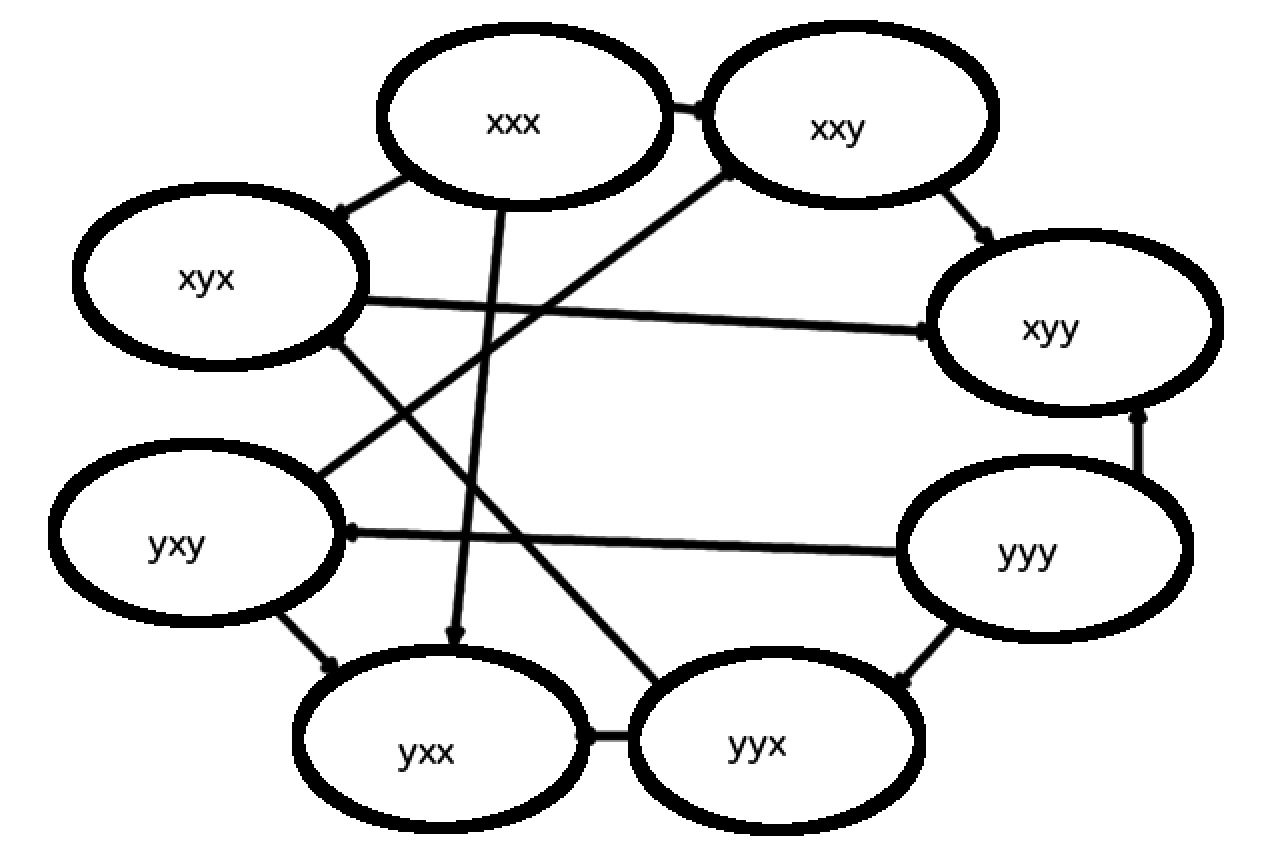
\includegraphics[width=10cm]{f1}
  \end{center}
  \end{figure}

  \item{What are the N.E.?}
  $yyy$ and $xxx$ are the NE.

  \item{If we apply log-linear learning, what is analytical stationary distrobution for
    $T=10$, $T=1$, and $T=0.1$?}\\
  Since this is a potential game, we know that there will only be one stationary distrobution.
  At $T=10$ this looks like:
  \[
    p_i=\frac{e^{\frac{1}{T}u_i(a_i)}}{\sum_{\tilde{a}\in\mathcal{A}_i}e^{\frac{1}{T}u_i(\tilde{a},a_{-i})}}
  \]
  So if we are at $xxx$, then player 1 will see the following:
  \[
    p_1(x) = \frac{e^{\frac{1}{10}3/4}}{e^{\frac{1}{10}3/4}+e^{\frac{1}{10}0}} = 0.52
  \]
  and indeed for all players:
  \[
    p = \left(
      \begin{array}{c}
        .5187 \\
        .5125 \\
        .5187
      \end{array}
    \right)
  \]
  for $T=1$:
  \[
    p = \left(
      \begin{array}{c}
        .6792 \\
        .6225 \\
        .6792
      \end{array}
    \right)
  \]
  and for $T=0.1$:
  \[
    p = \left(
      \begin{array}{c}
        .9994 \\
        .9933 \\
        .9994
      \end{array}
    \right)
  \]
And as $t\rightarrow0$ the stationary distrobution becomes $\left(
      \begin{array}{c}
        1 \\
        0
      \end{array}
    \right)$ for all players.
\end{enumerate}

\textbf{Part \#2:} Model the above mutiagent system as a game with player set $\mathcal{V}$ and the
Shapley value utility.

\begin{enumerate}[(a)]
  \item{What is the payoff matrix?}\\
  We know that a utility for a specific player will look like:
  \[
    U_i(a) = \sum_{r\in a_i} \sum_{T \subseteq \{a\}_r \backslash\{i\}}\frac{|T|!(|a|_r-|T|-1)!}{(|a|_r)!}(W_r(T \cup \{i\}) - W_r(T))
  \]
  We will calculate these when we get to the numeric values.

\item{From this point on, i.e., all future questions in Part \#2, set $v_x=2$, $v_y=1$, $p_1=1$,
    $p_2 = 1/2$, and $p_3 = 1/4$.  What is the payoff matrix for this specific setting?}\\
  We can now find the payoff matrix:
  \begin{center}
  \begin{tabular}{r |c|c|}
    \multicolumn{1}{r}{}
    & \multicolumn{1}{c}{$x$}
    & \multicolumn{1}{c}{$y$}\\
    \cline{2-3}
    $x$ & 4/3, 11/24, 5/24 & 1, 1/2, 1\\
    \cline{2-3}
    $y$ & 1, 5/8, 5/8 & 1/2, 1/2, 1/2\\
    \cline{2-3}
  \end{tabular}
  \begin{tabular}{r |c|c|}
    \multicolumn{1}{r}{}
    & \multicolumn{1}{c}{$x$}
    & \multicolumn{1}{c}{$y$}\\
    \cline{2-3}
    $x$ & 1, 1, 1/4 & 2, 5/16, 5/16\\
    \cline{2-3}
    $y$ & 1/2, 1, 1/2 & 2/3, 11/48, 5/48\\
    \cline{2-3}
  \end{tabular}\\
  \vspace{2mm}
  \hspace{6mm}$x$\hspace{5.4cm}$y$\\
  \end{center}

  \item{Is the game a potential game? If so, what is the potential function? (Hint: Set $\Phi(x,x,x)=0$).}

  \begin{center}
  \begin{tabular}{r |c|c|}
    \multicolumn{1}{r}{}
    & \multicolumn{1}{c}{$x$}
    & \multicolumn{1}{c}{$y$}\\
    \cline{2-3}
    $x$ & 0 & 1/24\\
    \cline{2-3}
    $y$ & -1/3 & -1/8\\
    \cline{2-3}
  \end{tabular}
  \begin{tabular}{r |c|c|}
    \multicolumn{1}{r}{}
    & \multicolumn{1}{c}{$x$}
    & \multicolumn{1}{c}{$y$}\\
    \cline{2-3}
    $x$ & 1/24 & x\\
    \cline{2-3}
    $y$ & x & x\\
    \cline{2-3}
  \end{tabular}\\
  \vspace{2mm}
  \hspace{6mm}$x$\hspace{5.4cm}$y$\\
  \end{center}

\end{enumerate}

\end{document}
